\documentclass[a4paper]{article}

%use the english line for english reports
%usepackage[english]{babel}
\usepackage[portuguese]{babel}
\usepackage[utf8]{inputenc}
\usepackage{indentfirst}
\usepackage{graphicx}
\usepackage{verbatim}


\begin{document}

\setlength{\textwidth}{16cm}
\setlength{\textheight}{22cm}

\title{\Huge\textbf{Game of Soldiers - 16!}\linebreak\linebreak\linebreak
\Large\textbf{Relatório Intercalar}\linebreak\linebreak
\linebreak\linebreak

\includegraphics[scale=0.1]{feup-logo.png}\linebreak\linebreak
\linebreak\linebreak
\Large{Mestrado Integrado em Engenharia Informática e Computação} \linebreak\linebreak
\Large{Programação em Lógica}\linebreak
}

\author{\textbf{Grupo 16!\_1:}\\
João Soares Correia - 201101753 \\
Filipe Diogo Soares Eiras - 201103055 \\
\linebreak\linebreak \\
 \\ Faculdade de Engenharia da Universidade do Porto \\ Rua Roberto Frias, s\/n, 4200-465 Porto, Portugal \linebreak\linebreak\linebreak
\linebreak\linebreak\vspace{1cm}}

\maketitle
\thispagestyle{empty}

%************************************************************************************************
%************************************************************************************************

\newpage

%Todas as figuras devem ser referidas no texto. %\ref{fig:codigoFigura}
%
%%Exemplo de código para inserção de figuras
%%\begin{figure}[h!]
%%\begin{center}
%%escolher entre uma das seguintes três linhas:
%%\includegraphics[height=20cm,width=15cm]{path relativo da imagem}
%%\includegraphics[scale=0.5]{path relativo da imagem}
%%\includegraphics{path relativo da imagem}
%%\caption{legenda da figura}
%%\label{fig:codigoFigura}
%%\end{center}
%%\end{figure}
%
%
%\textit{Para escrever em itálico}
%\textbf{Para escrever em negrito}
%Para escrever em letra normal
%``Para escrever texto entre aspas''
%
%Para fazer parágrafo, deixar uma linha em branco.
%
%Como fazer bullet points:
%\begin{itemize}
	%\item Item1
	%\item Item2
%\end{itemize}
%
%Como enumerar itens:
%\begin{enumerate}
	%\item Item 1
	%\item Item 2
%\end{enumerate}
%
%\begin{quote}``Isto é uma citação''\end{quote}


%%%%%%%%%%%%%%%%%%%%%%%%%%
\section{O Jogo 16!}

O jogo 16!, da autoria de Niek Neuwahl, é um jogo constituido por 16 peças todas diferentes, cada uma dividida num quadrado 3X3, com um número crescente de pontos até um máximo de 8.

\begin{figure}[h!]
  \centering
      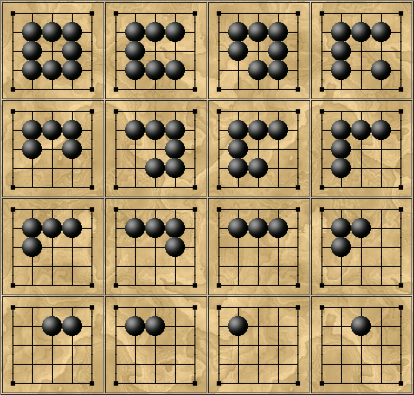
\includegraphics[width=0.5\textwidth]{Pieces}
  \caption{Exemplo das 16 peças do jogo.}
\end{figure}

Estas peças são colocadas em cima de um tabuleiro quadrado 12X12.

\begin{figure}[h!]
  \centering
      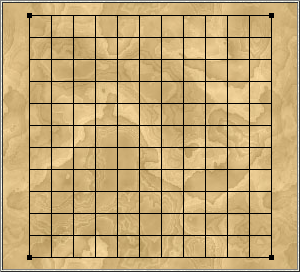
\includegraphics[width=0.5\textwidth]{Board}
  \caption{Exemplo dao tabuleiro.}
\end{figure}

Deste modo podemos ver o tabuleiro como conjunto 4X4 de àreas 3X3 onde o jogador coloca as peças.

\subsection{Como jogar:}

As peças devem ser colocadas numa das àreas 4X4, de modo a que 2 peças se encostem os pontos e os vazios correspondem uma com a outra.

\begin{figure}[h!]
  \centering
      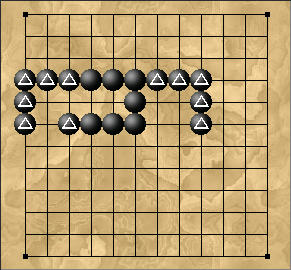
\includegraphics[width=0.5\textwidth]{Example}
  \caption{Exemplo de uma jogada. Do lado esquerdo a jogada é permitida, do lado direito não.}
\end{figure}

\subsection{Jogo: 1 Jogador:}

Tentar completar o tabuleiro usando todas as peças.

\subsection{Jogo: 2 Jogadores:}

Depois de se colocar uma peça numa das 4 àreas centrais, todas as peças estão com a face voltada para cima. À vez cada jogador pega numa peça e coloca-a em contacto com uma ou mais peças já colocadas. Perde o jogador que não conseguir jogar no seu turno.

\subsection{Jogo: Mais Jogadores:}

A cada seu turno, cada jogador baralha as peças e empilha-as voltadas para cima. Pega na primeira peça e coloca-a à sua frente. A seguir pega na segunda peça e tenta encaixa-la com a anterior. E continua enquanto conseguir encaixar as peças até um máximo de 4X4 peças. Quando não conseguir pára. A sua pontuação é o seu número máximo de peças. Ganha quem tiver a maior pontuação. Se a segunda peça não encaixar na primeira, o jogador pode colocar esta no fim da pilha e usar a terceira peça.

%%%%%%%%%%%%%%%%%%%%%%%%%%
\section{Representação do Estado do Jogo}

Descrever a forma de representação do estado do tabuleiro (tipicamente uma lista de listas), com exemplificação em Prolog de posições iniciais do jogo, posições intermédias e finais, acompanhadas de imagens ilustrativas.


%%%%%%%%%%%%%%%%%%%%%%%%%%
\section{Visualização do Tabuleiro}

Descrever a forma de visualização do tabuleiro em modo de texto e o(s) predicado(s) Prolog construídos para o efeito.
Deve ser incluída pelo menos uma imagem correspondente ao output produzido pelo predicado de visualização.


%%%%%%%%%%%%%%%%%%%%%%%%%%
\section{Movimentos}

Elencar os movimentos (tipos de jogadas) possíveis e definir os cabeçalhos dos predicados que serão utilizados (ainda não precisam de estar implementados).


\end{document}
